% Neso videos: GCD by the Euclidean algorithm, method 1 (table) and method 2 (recursive) (notes9.md); college Lecture 2
% (divisibility, gcd, Euclid); Forouzan 2.1. Every number recomputed by script (scratchpad/r4/verify.py).
\section{GCD and the Euclidean Algorithm}\label{sec:gcd}

The previous section showed that $a$ is invertible modulo $n$ exactly when $\gcd(a, n) = 1$, and that $ax \equiv b \pmod n$ is solvable exactly when $\gcd(a, n)$ divides $b$. Cryptography therefore keeps asking for greatest common divisors: is the Hill key's determinant co-prime to 26, is the RSA exponent $e$ co-prime to $\phi(n)$, does a congruence have a solution. The school method, factorising both numbers, is useless here, because factoring large numbers is exactly the problem RSA relies on being infeasible. Euclid's algorithm (about 300 BC) computes the gcd using only divisions with remainder, and its number of steps grows with the number of digits rather than with the size of the numbers. Its extension in the next section also produces the inverse.

\subsection{Divisibility and common divisors}
If $a = q \times n$ for some integer $q$, that is, if dividing $a$ by $n$ leaves remainder 0, then $n$ \textbf{divides} $a$, written $n \mid a$, and $n$ is a \emph{divisor} (factor) of $a$. For example $4 \mid 32$, while $8 \nmid 42$ because $42 = 5 \times 8 + 2$. Lecture 2 lists four properties, and each follows from the definition in one line.
\begin{itemize}[leftmargin=1.5em]
  \item \textbf{Property 1:} if $a \mid 1$, then $a = \pm 1$, since no other integer divides 1.
  \item \textbf{Property 2:} if $a \mid b$ and $b \mid a$, then $a = \pm b$. Write $b = ka$ and $a = lb$; then $a = lka$, so $lk = 1$ and $k = l = \pm 1$ (for $a \ne 0$).
  \item \textbf{Property 3 (transitivity):} if $a \mid b$ and $b \mid c$, then $a \mid c$, because $b = ka$ and $c = lb$ give $c = (lk)a$. For example $3 \mid 15$ and $15 \mid 45$, so $3 \mid 45$.
  \item \textbf{Property 4 (linear combinations):} if $a \mid b$ and $a \mid c$, then $a \mid (mb + nc)$ for all integers $m, n$, because $b = ka$ and $c = la$ give $mb + nc = (mk + nl)a$. For example $3 \mid 15$ and $3 \mid 9$, so $3 \mid (2 \times 15 + 4 \times 9) = 66$.
\end{itemize}
Property 4 is the engine of Euclid's algorithm, and it is also behind every ``no solution'' argument in this chapter: a common divisor of $a$ and $n$ divides every combination $ax + ny$.

Every positive integer has 1 and itself as divisors. A prime has exactly these two, and a composite number has more. \imp{The greatest common divisor $\gcd(a, b)$ of two positive integers is the largest integer that divides both}; it is also called the highest common factor (HCF). For small numbers it can be found by listing divisors. The slide's example is 140 and 12, whose common divisors are 1, 2 and 4, so $\gcd(140, 12) = 4$. The lecture video does the same for $\gcd(12, 33) = 3$ (common divisors $\{1, 3\}$), $\gcd(25, 150) = 25$ and $\gcd(13, 31) = 1$. Listing all divisors amounts to factoring, so the method cannot scale to cryptographic sizes.
\begin{center}
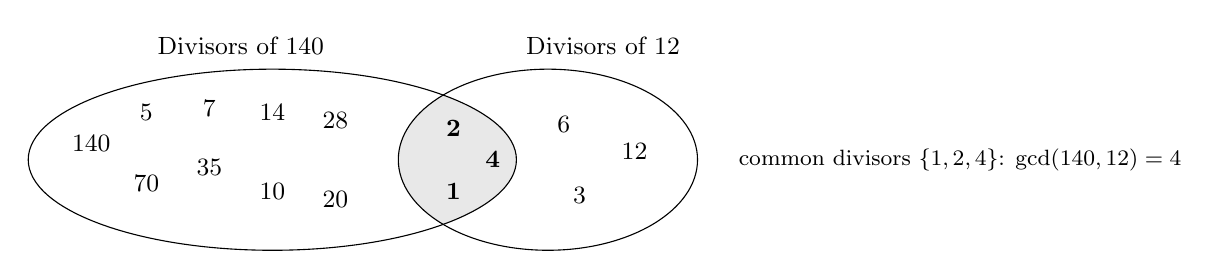
\begin{tikzpicture}[font=\small]
  \begin{scope}
    \clip (0,0) ellipse (3.1 and 1.15);
    \fill[gray!18] (3.5,0) ellipse (1.9 and 1.15);
  \end{scope}
  \draw (0,0) ellipse (3.1 and 1.15);
  \draw (3.5,0) ellipse (1.9 and 1.15);
  \node at (-0.4,1.45) {Divisors of 140};
  \node at (4.2,1.45) {Divisors of 12};
  \foreach \x/\y/\v in {-2.3/0.2/140,-1.6/0.6/5,-1.6/-0.3/70,-0.8/0.65/7,-0.8/-0.1/35,0/0.6/14,0/-0.4/10,0.8/0.5/28,0.8/-0.5/20}{\node at (\x,\y) {\v};}
  \foreach \x/\y/\v in {2.3/0.4/2,2.3/-0.4/1,2.8/0/4}{\node[font=\small\bfseries] at (\x,\y) {\v};}
  \foreach \x/\y/\v in {3.7/0.45/6,3.9/-0.45/3,4.6/0.1/12}{\node at (\x,\y) {\v};}
  \node[anchor=west] at (5.8,0) {\footnotesize common divisors $\{1, 2, 4\}$: $\gcd(140, 12) = 4$};
\end{tikzpicture}
\end{center}

\subsection{Euclid's algorithm and why it works}
The algorithm rests on two facts stated on the slides.
\[
\textbf{Fact 1: } \gcd(a, 0) = a, \qquad\qquad \textbf{Fact 2: } \gcd(a, b) = \gcd(b, r), \text{ where } r = a \bmod b .
\]
\textbf{Why Fact 1 holds.} Every integer divides 0 (since $0 = 0 \times d$), so the common divisors of $a$ and 0 are just the divisors of $a$, and the largest of these is $a$ itself.

\textbf{Why Fact 2 holds.} Divide: $a = qb + r$. If $d$ divides both $a$ and $b$, then by Property 4 it divides $a - qb = r$. Conversely, if $d$ divides both $b$ and $r$, then it divides $qb + r = a$. The pairs $(a, b)$ and $(b, r)$ therefore have exactly the same set of common divisors, and so the same greatest common divisor. The argument works for any multiple $qb$; the remainder is used because it makes the new pair as small as possible.

\textbf{The algorithm.} Apply Fact 2 repeatedly, replacing $(a, b)$ by $(b, a \bmod b)$, until the second number is 0; then Fact 1 gives the answer. The slide's example:
\[
\gcd(36, 10) = \gcd(10, 6) = \gcd(6, 4) = \gcd(4, 2) = \gcd(2, 0) = \mathbf{2}.
\]
\textbf{Termination.} Each step replaces the second number $b$ by $r = a \bmod b$, and $0 \le r < b$. The second numbers therefore form a strictly decreasing sequence of non-negative integers, $b > r_1 > r_2 > \cdots$, which must reach 0 after at most $b$ steps; the last non-zero term is the gcd.

\textbf{Speed.} The bound of $b$ steps is far too pessimistic: the remainder at least halves every two steps. Consider three consecutive remainders, where $r_{i+2} = r_i \bmod r_{i+1}$. If $r_{i+1} \le r_i / 2$, then $r_{i+2} < r_{i+1} \le r_i / 2$. Otherwise $r_{i+1} > r_i / 2$, the quotient is 1, and $r_{i+2} = r_i - r_{i+1} < r_i / 2$. Either way two steps halve the remainder, so at most about $2\log_2 b$ divisions are needed, which is linear in the number of digits. A 1024-bit $b$ therefore needs at most about 2048 divisions, while listing divisors would need about $2^{1024}$ trial divisions. The slowest inputs are consecutive Fibonacci numbers, where every quotient is 1: $\gcd(89, 55)$ takes 9 divisions.

Forouzan writes the algorithm with two variables $r_1$ and $r_2$ that hold the current pair:
\begin{center}
\begin{minipage}{0.55\textwidth}
\small\ttfamily
r$_1$ $\leftarrow$ a;\quad r$_2$ $\leftarrow$ b;\hfill\textrm{(initialisation)}\\
while (r$_2$ > 0)\\
\{\\
\hspace*{1.5em}q $\leftarrow$ r$_1$ / r$_2$;\hfill\textrm{(integer quotient)}\\
\hspace*{1.5em}r $\leftarrow$ r$_1$ $-$ q $\times$ r$_2$;\\
\hspace*{1.5em}r$_1$ $\leftarrow$ r$_2$;\quad r$_2$ $\leftarrow$ r;\\
\}\\
gcd(a, b) $\leftarrow$ r$_1$
\end{minipage}
\end{center}

\begin{mustknow}
$\gcd(a, b) = \gcd(b,\ a \bmod b)$ and $\gcd(a, 0) = a$. Divide, shift ($B \to A$, $R \to B$), and stop when the second number is 0: the gcd is the last non-zero remainder. At most about $2\log_2 b$ divisions.
\end{mustknow}

\subsection{Method 1: the table (Q, A, B, R)}
The lecture video lays the divisions out as a table, which is the format to use in an exam.
\begin{enumerate}[leftmargin=1.5em,itemsep=1pt]
  \item Draw the columns $Q$ (quotient), $A$, $B$ and $R$ (remainder), and start with $A$ = the larger number and $B$ = the smaller.
  \item In each row compute $Q = \lfloor A/B \rfloor$ and $R = A \bmod B$, so that $A = Q \times B + R$.
  \item In the next row $B$ moves into $A$ and $R$ moves into $B$ (the diagonal arrows below). This is Fact 2.
  \item Stop when $B = 0$, since division by 0 is impossible; write X for $Q$ and $R$. The gcd is the $A$ of that row (Fact 1).
\end{enumerate}
\begin{center}
\begin{tikzpicture}[x=11mm,y=6mm]
  \foreach \h [count=\c] in {Q,A,B,R}{\node[font=\small\bfseries] at (\c,0) {\h};}
  \draw (0.5,-0.5) -- (4.5,-0.5);
  \foreach \q/\a/\b/\r [count=\i] in {2/33/12/9, 1/12/9/3, 3/9/3/0, X/3/0/X}{
    \node[font=\small] at (1,-\i) {\q};
    \node[font=\small] (a\i) at (2,-\i) {\a};
    \node[font=\small] (b\i) at (3,-\i) {\b};
    \node[font=\small] (r\i) at (4,-\i) {\r};
  }
  \foreach \i in {1,2,3}{\pgfmathtruncatemacro{\j}{\i+1}
    \draw[-{Stealth[length=1.5mm]},orange!80!black] (b\i.south west) -- (a\j.north east);
    \draw[-{Stealth[length=1.5mm]},orange!80!black] (r\i.south west) -- (b\j.north east);}
  \draw[warn,thick,dashed,rounded corners=2pt] (1.6,-3.6) rectangle (2.4,-4.4);
  \node[font=\small,anchor=west] at (4.8,-1) {$33 = 2\cdot12 + 9$};
  \node[font=\small,anchor=west] at (4.8,-2) {$12 = 1\cdot9 + 3$};
  \node[font=\small,anchor=west] at (4.8,-3) {$9 = 3\cdot3 + 0$ \;(don't stop yet!)};
  \node[font=\small,anchor=west] at (4.8,-4) {$B = 0$: stop. \;$\gcd(12, 33) = \mathbf{3}$};
\end{tikzpicture}
\end{center}
The other lecture examples, and Forouzan's slide example with the columns named $q, r_1, r_2, r$ (the same table under different names):
\begin{center}\small
\begin{minipage}[t]{0.27\textwidth}
\centering
$\gcd(750, 900)$\\[2pt]
\begin{tabular}{cccc}
\toprule
Q&A&B&R\\
\midrule
1&900&750&150\\
5&750&150&0\\
X&\textbf{150}&0&X\\
\bottomrule
\end{tabular}
\end{minipage}\hfill
\begin{minipage}[t]{0.27\textwidth}
\centering
$\gcd(252, 105)$\\[2pt]
\begin{tabular}{cccc}
\toprule
Q&A&B&R\\
\midrule
2&252&105&42\\
2&105&42&21\\
2&42&21&0\\
X&\textbf{21}&0&X\\
\bottomrule
\end{tabular}
\end{minipage}\hfill
\begin{minipage}[t]{0.36\textwidth}
\centering
$\gcd(2740, 1760)$ (Lecture 2)\\[2pt]
\begin{tabular}{cccc}
\toprule
$q$&$r_1$&$r_2$&$r$\\
\midrule
1&2740&1760&980\\
1&1760&980&780\\
1&980&780&200\\
3&780&200&180\\
1&200&180&20\\
9&180&20&0\\
&\textbf{20}&0&\\
\bottomrule
\end{tabular}
\end{minipage}
\end{center}
\textbf{Shortcut.} The gcd is the \textbf{last non-zero remainder} (9, 3, \textbf{3}, then 0; or 42, \textbf{21}, then 0). The extra row with $B = 0$ is only where the lecture reads it off. The Lecture 2 class exercise, $\gcd(25, 60)$, runs $60 = 2 \times 25 + 10$, $25 = 2 \times 10 + 5$, $10 = 2 \times 5 + 0$, giving $\mathbf{5}$.

\subsection{Method 2: recursion}
Facts 1 and 2 are already a recursive definition, and the second lecture video writes them as a function:
\begin{center}
\begin{minipage}{0.45\textwidth}
\small\ttfamily
Prerequisite: a > b\\
Euclid\_GCD(a, b):\\
\hspace*{1.5em}if b = 0 then\\
\hspace*{3em}return a;\hfill\textrm{(Fact 1)}\\
\hspace*{1.5em}else\\
\hspace*{3em}return Euclid\_GCD(b, a mod b);\hfill\textrm{(Fact 2)}
\end{minipage}
\end{center}
\begin{minipage}[t]{0.42\textwidth}
\small
\textbf{$\gcd(50, 12)$}\\
$= \gcd(12, 50 \bmod 12) = \gcd(12, 2)$\\
$= \gcd(2, 12 \bmod 2) = \gcd(2, 0)$\\
$= \mathbf{2}$
\end{minipage}\hfill
\begin{minipage}[t]{0.55\textwidth}
\small
\textbf{$\gcd(83, 19)$}\\
$= \gcd(19, 7)$ \quad ($83 = 4\cdot19 + 7$)\\
$= \gcd(7, 5)$ \quad ($19 = 2\cdot7 + 5$)\\
$= \gcd(5, 2)$ \quad ($7 = 1\cdot5 + 2$)\\
$= \gcd(2, 1)$ \quad ($5 = 2\cdot2 + 1$)\\
$= \gcd(1, 0) = \mathbf{1}$ \quad ($2 = 2\cdot1 + 0$)
\end{minipage}

\medskip
Both methods perform exactly the same divisions, so either may be used. The prerequisite $a > b$ is a convenience, not a necessity. If the smaller number comes first, the first call swaps them at the cost of one wasted step: $\gcd(12, 33) \to \gcd(33, 12 \bmod 33) = \gcd(33, 12)$, since $12 \bmod 33 = 12$. In the exam it is cleaner to write the larger number first.

\subsection{Relatively prime numbers}
\imp{Two integers $a$ and $b$ are relatively prime (co-prime) if $\gcd(a, b) = 1$}, as for 83 and 19 above. The condition is about the pair: neither number has to be prime, as $\gcd(8, 9) = 1$ shows. Cryptography needs the notion for three reasons. First, $a^{-1} \bmod n$ exists only if $\gcd(a, n) = 1$ (\S\ref{sec:modular}); this is the Hill key condition $\gcd(\det K, 26) = 1$ and the affine-cipher condition on the multiplier. Second, RSA key generation chooses $e$ with $\gcd(e, \phi(n)) = 1$, so that $d = e^{-1} \bmod \phi(n)$ exists. Third, the number of residues co-prime to $n$ is Euler's totient $\phi(n)$ (\S\ref{sec:totient}). Euclid's algorithm decides co-primality; the extended algorithm (\S\ref{sec:exteuclid}) runs the same divisions while tracking two extra columns and produces the inverse itself, instead of the trial-and-error table used for $23^{-1} \bmod 26$ in the Hill cipher.

\begin{worked}[: GCD by the Euclidean algorithm (Forouzan exercise)]
\textbf{Q.} Find (a) $\gcd(88, 220)$ \quad (b) $\gcd(300, 42)$ \quad (c) $\gcd(24, 320)$ \quad (d) $\gcd(401, 700)$. Which pairs are relatively prime?

\textbf{A.} Larger number first; each line is one row $A = Q \times B + R$.
\begin{center}\small
\begin{tabular}{@{}lll@{}}
\toprule
Pair & Divisions & gcd\\
\midrule
(a) 220, 88 & $220 = 2 \times 88 + 44$, \;$88 = 2 \times 44 + 0$ & \textbf{44}\\
(b) 300, 42 & $300 = 7 \times 42 + 6$, \;$42 = 7 \times 6 + 0$ & \textbf{6}\\
(c) 320, 24 & $320 = 13 \times 24 + 8$, \;$24 = 3 \times 8 + 0$ & \textbf{8}\\
\bottomrule
\end{tabular}
\end{center}
(d) needs a longer table:
\begin{center}\small
\begin{tabular}{cccc|l}
\toprule
Q&A&B&R&\\
\midrule
1&700&401&299&$700 = 1 \times 401 + 299$\\
1&401&299&102&$401 = 1 \times 299 + 102$\\
2&299&102&95&$299 = 2 \times 102 + 95$\\
1&102&95&7&$102 = 1 \times 95 + 7$\\
13&95&7&4&$95 = 13 \times 7 + 4$\\
1&7&4&3&$7 = 1 \times 4 + 3$\\
1&4&3&1&$4 = 1 \times 3 + 1$\\
3&3&1&0&$3 = 3 \times 1 + 0$\\
X&\textbf{1}&0&X&\\
\bottomrule
\end{tabular}
\end{center}
\textbf{Answers: 44, 6, 8, 1.} Only 401 and 700 are relatively prime, so 401 has an inverse modulo 700 and the other pairs have none. \textbf{Check:} $88 = 2 \times 44$ and $220 = 5 \times 44$ with $\gcd(2, 5) = 1$; similarly $300 = 50 \times 6$, $42 = 7 \times 6$ and $320 = 40 \times 8$, $24 = 3 \times 8$, with co-prime cofactors.
\end{worked}

\textbf{Lecture homework:} $\gcd(1005, 105)$ (table method) and $\gcd(529, 123)$ (recursive method). Solutions are in practice Q43.

\begin{trap}[: reading the table]
\begin{itemize}[leftmargin=1.5em]
  \item Stop when $B = 0$, not when $R = 0$. In the row where $R$ first becomes 0, the answer is that row's $B$, which moves into $A$ in the next row; reading $A$ from the row with $R = 0$ gives a wrong answer (9 instead of 3 for $\gcd(33, 12)$).
  \item Swapping the meaning of the two outputs: ``$A \bmod B$'' gives the remainder $R$, while ``$A$ divided by $B$'' gives the quotient $Q$. The table needs both.
  \item Show every division as $A = Q \times B + R$ in the exam; the marks are for the steps, not only for the final number.
\end{itemize}
\end{trap}

\begin{fixbox}
\begin{itemize}
  \item All results are correct (checked by script): 3, 25, 1, 3, 150, 21, 2, 1 from the videos, and $\gcd(36, 10) = 2$, $\gcd(2740, 1760) = 20$, $\gcd(25, 60) = 5$, $\gcd(140, 12) = 4$ from the Lecture 2 slides.
  \item Verbal slips only: ``divisors of 13'' means 33 (video 1); ``a = 9'' means 19 (video 2). The slides are right.
  \item Wording: ``$A$ mod $B$'' gives the \emph{remainder}; ``$A$ divided by $B$'' gives the quotient $Q$. The table needs both.
\end{itemize}
\end{fixbox}
